\usetikzlibrary{quotes,angles}
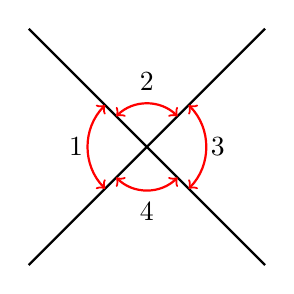
\begin{tikzpicture}[scale=1.5]
  %
  \coordinate (a) at (-1,1);
  \coordinate (o) at (0,0) ;
  \coordinate (b) at (1,-1);
  \coordinate (d) at (1,1);
  \coordinate (e) at (-1,-1);
  %
  \draw[thick] (a) -- (b);
  \draw[thick] (e) -- (d);
  %
   \draw pic["$1$", thick, draw=red, <->, angle eccentricity=1.2, angle radius=0.75cm] {angle=a--o--e};
   \draw pic["$2$", thick, draw=red, <->, angle eccentricity=1.5, angle radius=0.55cm] {angle=d--o--a};
   \draw pic["$3$", thick, draw=red, <->, angle eccentricity=1.2, angle radius=0.75cm] {angle=b--o--d};
   \draw pic["$4$", thick, draw=red, <->, angle eccentricity=1.5, angle radius=0.55cm] {angle=e--o--b};
   %
\end{tikzpicture}